\subsection{Short term analysis}

\subsubsection{Negative news}

\subsubsection{Positive news}

\subsection{Long term analysis}



\subsubsection{Negative news}


  However, the amount of firms in the portfolios does also have implication for the validity of the alpha, as the results indicate that the numerical value of the alpha is not a sole determinant of whether abnormal performance has been detected. A reason could be that a low amount of average firms , e.g. 5 ($T = 1$ and 3 sd), 

A strict event criteria of 3 SDs presents relatively large negative alphas

  ??

  \subsubsection{Positive news}




\begin{figure} [H]
    \centering
    \caption{SDG 5 pillars: negative news}
    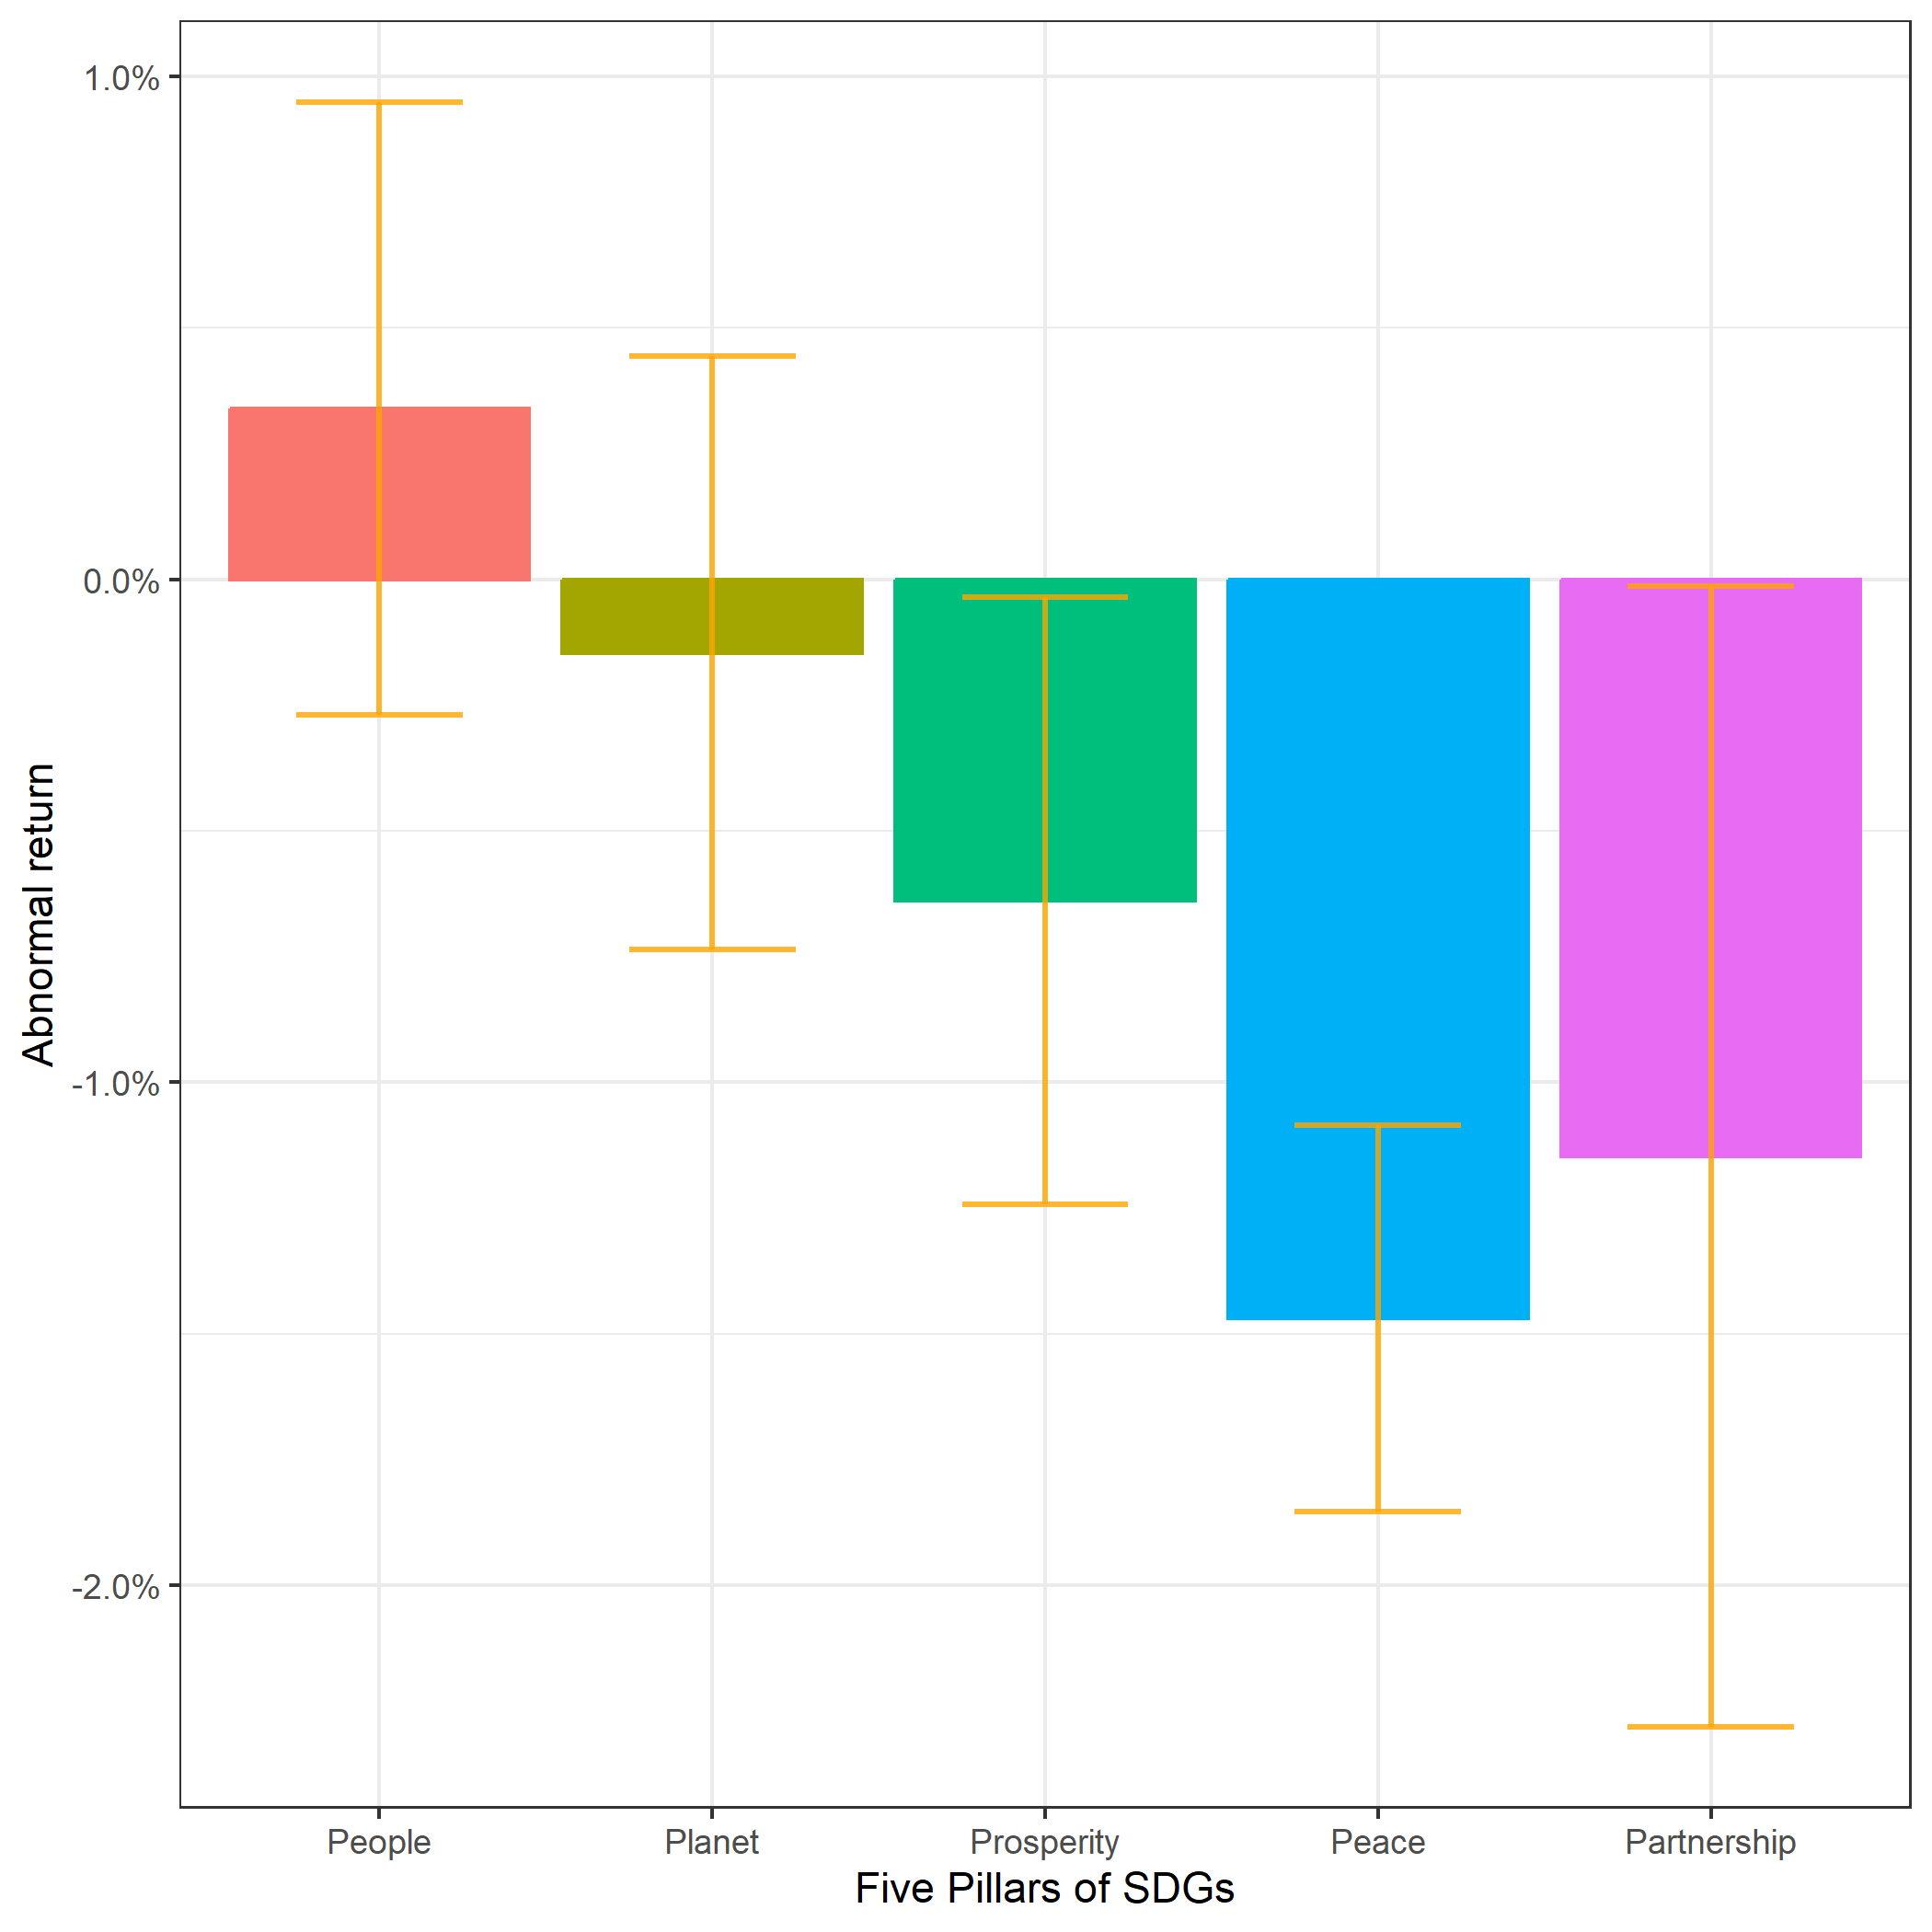
\includegraphics[scale=0.6]{Projekt/1.Figures analysis/ST_negative_sdg_bar_groups_0.png}
    \caption*{\footnotesize The figure illustrates the CAAR on $t = 10$ (the full period) from negative news. The error bars represent the 95\% confidence intervals of the CAAR.}
    \label{fig:ST_neg_bar}
\end{figure}



\begin{figure} [H]
    \centering
    \caption{SDG 5 pillars: positive news}
    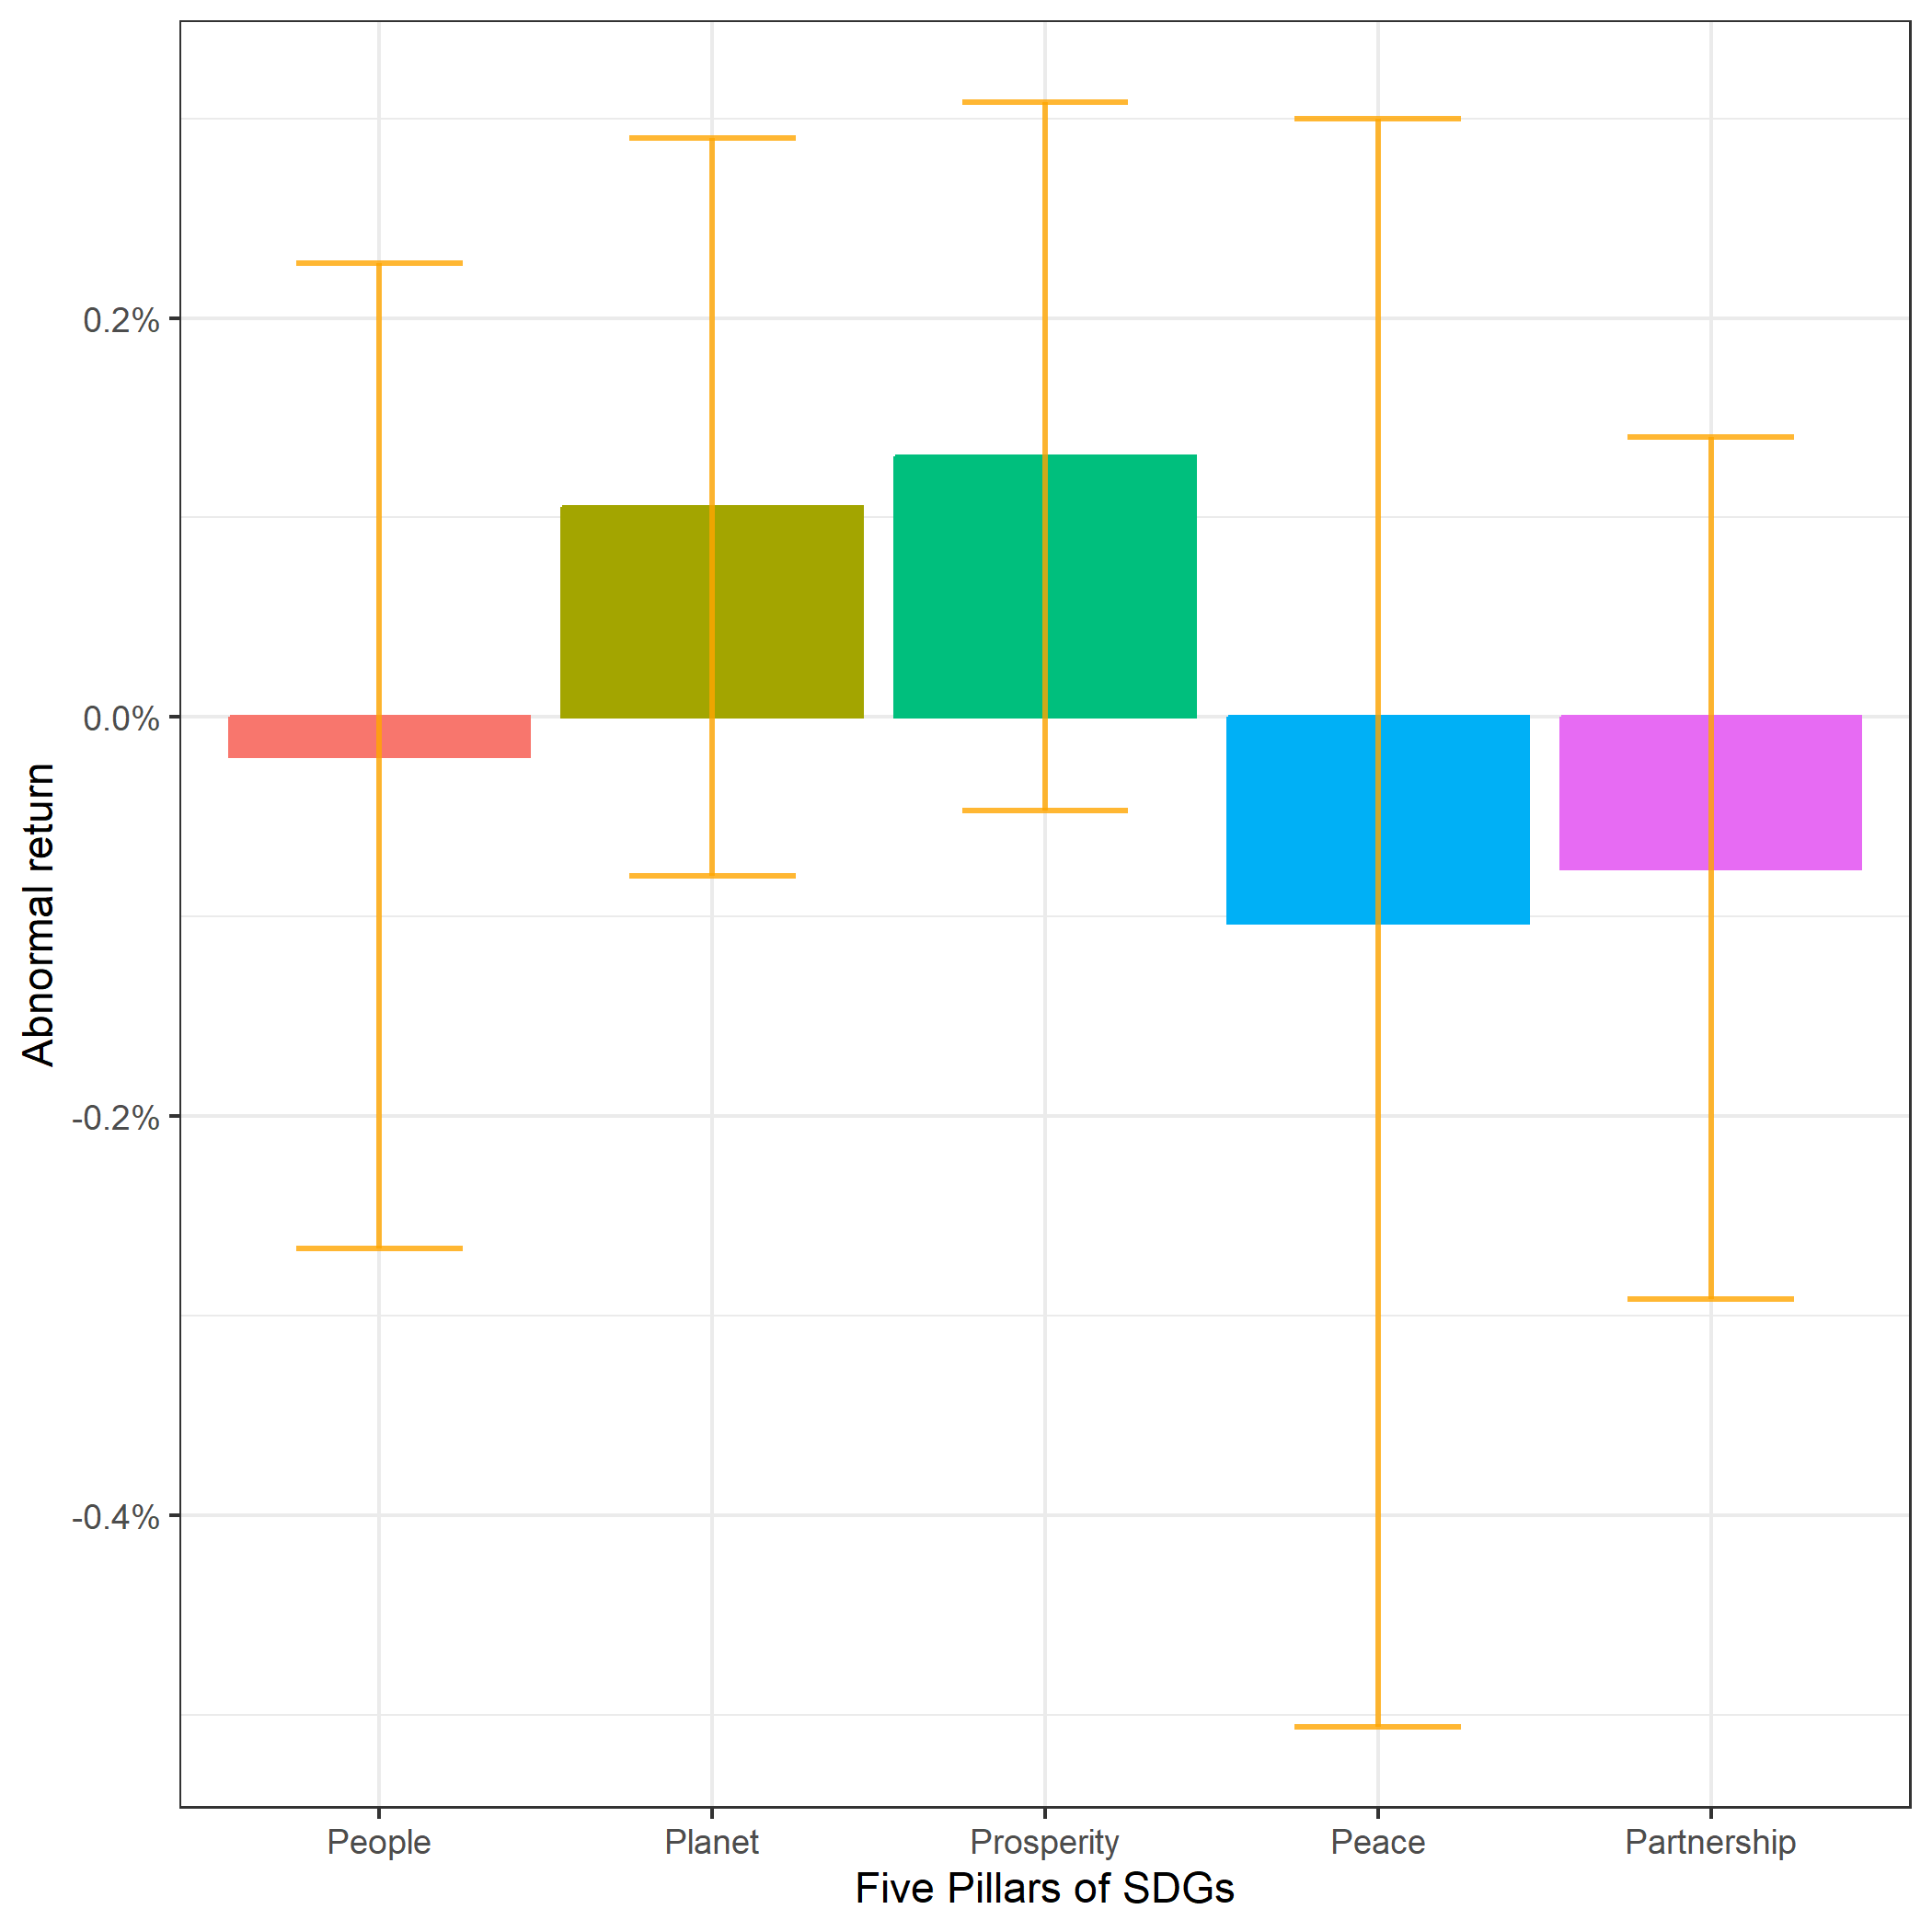
\includegraphics[scale=0.6]{Projekt/1.Figures analysis/ST_positive_sdg_bar_groups_0.png}
    \caption*{\footnotesize The figure illustrates the CAAR on $t = 10$ (full period) from positive news. The error bars represent the 95\% confidence intervals of the CAAR.}
    \label{fig:ST_pos_bar}
\end{figure}